\documentclass{standalone}
\usepackage{tikz}

\begin{document}
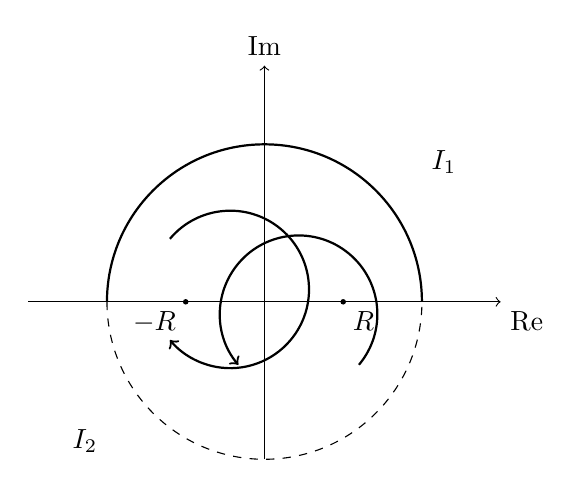
\begin{tikzpicture}

% 軸
\draw[->] (-3,0) -- (3,0) node[below right] {Re};
\draw[->] (0,-2) -- (0,3) node[above] {Im};

% 半円経路
\draw[thick] (-2,0) arc[start angle=180, end angle=0, radius=2];
\draw[dashed] (-2,0) arc[start angle=180, end angle=360, radius=2];

% 円内部
\draw[thick,->] (-1.2,0.8) arc[start angle=140, end angle=-140, radius=1];
\draw[thick,->] (1.2,-0.8) arc[start angle=-40, end angle=220, radius=1];

% 矢印の経路ラベル
\node[above right] at (2,1.5) {$I_1$};
\node[below left] at (-2,-1.5) {$I_2$};

% 点と円のマーク
\fill (1,0) circle(1pt) node[below right] {$R$};
\fill (-1,0) circle(1pt) node[below left] {$-R$};

\end{tikzpicture}
\end{document}
